

\chapter{Benchmarking of Asynchronous Data Processing Algorithms}
\label{cha:a_short_latex_tutorial_with_examples}

In this chapter, we delve into the benchmark results of two key algorithms applied using various strategies and implementations. These algorithms can be understood as abstract representations of real-world tasks that involve processing large amounts of data asynchronously. The two main algorithms under consideration are:

\begin{enumerate}
\item Finding the largest word in a set of files
\item Grouping of words based on their sizes, known as the "group words" operation
\end{enumerate}

The "group word" operation identifies words within a specified size range in a dataset. The algorithm then returns a collection of these words, along with a count of their occurrences, and is particularly designed to output the most recurring words within the specified range. This operation presents an intriguing computational challenge as it requires efficient data retrieval, processing, and frequency analysis.

Conversely, finding the largest word in a set of files, although seemingly simple, becomes a non-trivial task when considering vast amounts of data.

The data used in these tests is a collection of text files from Project Gutenberg, a large digital library of thousands of free eBooks. Project Gutenberg offers a wide variety of books in different languages, and for this experiment, we used a random sample of hundreds of books, providing a diverse and challenging dataset for our implementations.

During the implementations, a conscious effort was made to keep the operation pipelines as similar as possible across the different technologies for each algorithm. This endeavor aimed to create a fair and representative evaluation of the behaviors of each technology. By maintaining consistency in pipeline operations, we can more accurately attribute performance differences to the underlying technology, rather than variations in the implemented code. This approach brings us closer to a true comparison of how each technology handles the challenges of asynchronous I/O data retrieval and processing.

In certain instances, particularly with Java, there was a need to incorporate external libraries for non-blocking asynchronous file retrieval. This requirement highlights the varying degrees of native support for these operations across programming environments. Some environments have native functions, while others rely heavily on third-party solutions. This aspect of the project mirrors the challenges often faced in real-world environments, where the necessity to adapt and find suitable solutions is a common part of the development process.

The implementations differ in the specific programming languages, libraries, and technologies they use. This allows us to evaluate the relative strengths and weaknesses of each approach and provides valuable insights into how these factors can affect performance.

After presenting and discussing each implementation and its results, we will be able to directly compare them. This will enable us to draw meaningful conclusions about the performance of the strategies and technologies when applied to the same task under the same conditions. Specifically, we are interested in how the performance of a given strategy or technology can vary across different programming frameworks when tasked with finding the largest word and executing the group word operation.


\section{Strategies}
\label{subsec:strategies}

The aim of this section is to define various strategies that we will be implementing across different languages and technologies. While some of these strategies can be used universally across all platforms, others are platform-specific due to the constraints of the environment.

\subsubsection{Reactive Extensions (Rx)}
\label{subsubsec:rx}
Reactive Extensions (Rx) is a library for composing asynchronous and event-based programs using observable sequences. This model promotes a focus on data streams and the propagation of change. Rx has implementations in several programming languages including .NET (Rx.NET), Java (RxJava), and JavaScript (RxJS).

\subsubsection{Reactor (Flux)}
\label{subsubsec:reactor_flux}
Reactor is a fourth-generation reactive library, based on the Reactive Streams specification, for building non-blocking applications on the JVM based on Java 8 and later. The Flux class, a Reactive Streams Publisher with reactive operators, emits 0 to N elements, and then completes (successfully or with an error).

\subsubsection{Blocking Reader in Streams}
\label{subsubsec:blocking_reader_streams}
This strategy uses Java's streams interface to read the data in a blocking manner. Due to the blocking nature of the I/O operations, this approach may lead to slower processing times as it has to wait for each I/O operation to complete.

\subsubsection{Multi-threading}
\label{subsubsec:multithread}
This strategy leverages multi-threading to process data concurrently. By distributing the work across multiple threads, it often results in improved performance, especially for CPU-bound tasks.

\subsubsection{Kotlin Flow}
\label{subsubsec:kotlin_flow}
In Kotlin, the concept of 'flows' is integral to the Coroutines library. A Flow is an asynchronous data stream that sequentially emits values and completes normally or with an exception.

\subsubsection{Concurrency}
\label{subsubsec:concurrency}
Concurrency is used in combination with several of the aforementioned strategies such as Kotlin Flow and Rx. Concurrency aims to improve the performance of data processing by executing multiple tasks in parallel.

\subsubsection{Baseline}
\label{subsubsec:baseline}
The Baseline strategy is a straightforward implementation without any pipelining or other overhead. It serves as a reference for comparison. This method may use traditional synchronous I/O operations and sequential processing.

These strategies will be applied to our chosen algorithms and implemented in the .NET, Java, and Kotlin environments. It's important to note that the aim is not to find the 'best' strategy but to demonstrate the relative strengths and weaknesses of each approach, how they can affect performance, and how they fit into different programming paradigms.



\section{.NET Implementation}
\label{sec:dotnet_implementation}



\subsubsection{Approaches Explanation}

\subsection{Sync Baseline}

The Sync Baseline approach is the most straightforward and is synchronous, meaning it processes one task at a time and waits for each operation to complete before moving on to the next. This strategy reads a file line by line and extracts the longest word from each line. It repeats this for each file in the directory.

\subsection{Async Blocking Read}

The Async Blocking Read approach applies asynchronous programming to read file content. This approach reads files in blocks, with each block being processed for its longest word. However, while it does use async/await, it does not truly take full advantage of asynchrony as it still blocks on the read operation to complete before processing the block. 

\subsection{Async Single Task}

The Async Single Task approach is an asynchronous version of the baseline strategy. It uses async and await keywords to allow other tasks to execute when the current one is waiting for I/O operations to complete, improving the overall performance of the program. It reads a file line by line, extracts the longest word from each line, and repeats this for each file in the directory. The processing of each file is wrapped in a separate Task, but the processing of the files is still done sequentially. 

\subsection{Async Baseline}

The Async Baseline approach is similar to the Async Single Task approach but with one major difference: the processing of files is done in parallel, meaning it doesn't wait for a file to be completely processed before starting to process the next file. This strategy allows for better utilization of system resources, especially when dealing with a large number of files. 

\subsection{Linq Sync}

The Linq Sync approach uses LINQ (Language Integrated Query) to process the files. It is a synchronous approach that utilizes the powerful querying capabilities of LINQ to read and process the files. Despite being synchronous, LINQ's declarative nature can lead to more readable and concise code.

\subsection{Async Enumerable}

The Async Enumerable approach uses the IAsyncEnumerable interface to asynchronously stream and process data as it becomes available, instead of waiting for all data to be available as with traditional enumerables. This strategy can provide a performance boost when dealing with large datasets.

\subsection{Rx}

The Rx approach uses the Reactive Extensions (Rx) library for .NET, which provides tools for composing asynchronous and event-based programs using observable sequences and LINQ-style query operators. Like Async Enumerable, it can also stream and process data as it becomes available.


\subsubsection{Biggest Word Results}
\label{subsubsec:biggest_word_results_cs}

\begin{table}[H]
    \centering
    \resizebox{\textwidth}{!}{%
    \begin{tabular}{|l|c|}
    \hline
    \textbf{Strategy} & \textbf{Processing Time Average (s)} \\ \hline
    Sync Baseline & 15.8 \\ \hline
    Multithread (Async Blocking Read) & 1.6 \\ \hline
    Async Baseline (Async Single Task) & 2.8 \\ \hline
    Linq Sync & 22.2 \\ \hline
    Async Enumerable & 30 \\ \hline
    Rx & 23 \\ \hline
    Rx Async File Read & 15 \\ \hline
    \end{tabular}%
    }
    \caption{Processing times for different strategies for "Find the biggest word".}
    \label{tab:biggest_word_results_cs_1}
\end{table}
    
\begin{figure}[H]
    \raggedright
    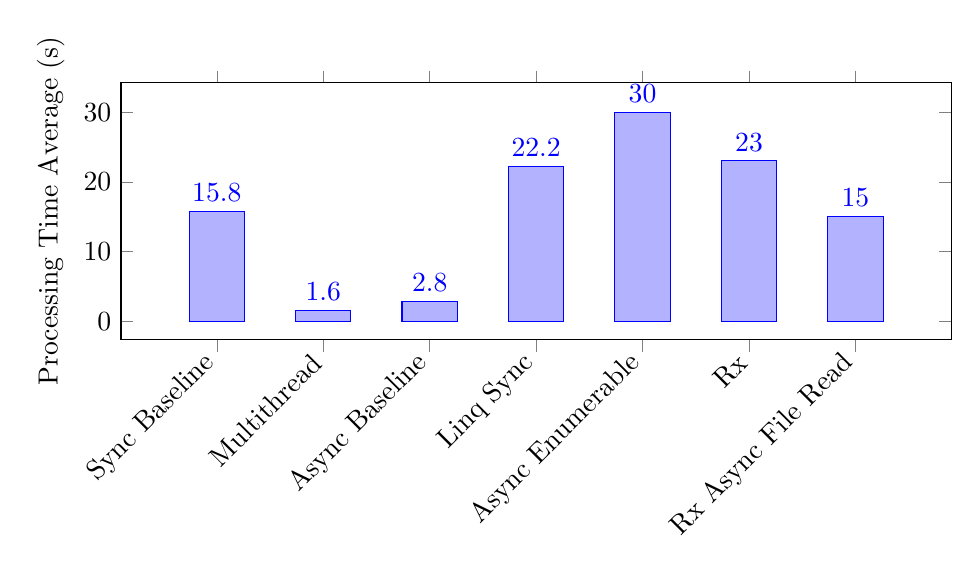
\begin{tikzpicture}
    \begin{axis}[
    ybar=2*\pgflinewidth,
    width=1.0\textwidth,
    height=0.4\textwidth,
    bar width=20pt,
    enlargelimits=0.15,
    legend style={at={(0.5,-0.2)}, anchor=north, legend columns=-1},
    ylabel={Processing Time Average (s)},
    symbolic x coords={Sync Baseline, Multithread, Async Baseline, Linq Sync, Async Enumerable, Rx, Rx Async File Read},
    xtick=data,
    xticklabel style={rotate=45,anchor=east},
    nodes near coords,
    nodes near coords align={vertical},
    ]
    \addplot coordinates {(Sync Baseline, 15.8) (Multithread, 1.6) (Async Baseline, 2.8) (Linq Sync, 22.2) (Async Enumerable, 30) (Rx, 23) (Rx Async File Read, 15)};
    \end{axis}
    \end{tikzpicture}
    \caption{Processing times for different strategies for "Find the biggest word".}
    \label{fig:biggest_word_results_cs_2}
\end{figure}


\subsubsection{Group Word Results}
\label{subsubsec:group_word_processing_times_cs}


\begin{table}[H]
    \centering
    \resizebox{\textwidth}{!}{%
    \begin{tabular}{|l|c|}
    \hline
    \textbf{Strategy} & \textbf{Processing Time Average (s)} \\ \hline
    RunCountWordsBaseline & 26 \\ \hline
    RunSyncTest & 22 \\ \hline
    RunAsyncEnumerableTest & 30 \\ \hline
    RunRxTest & 22 \\ \hline
    \end{tabular}%
    }
    \caption{Processing times for different strategies for "Count Words".}
    \label{tab:group_word_processing_times_cs}
\end{table}

\begin{figure}[H]
    \raggedright
    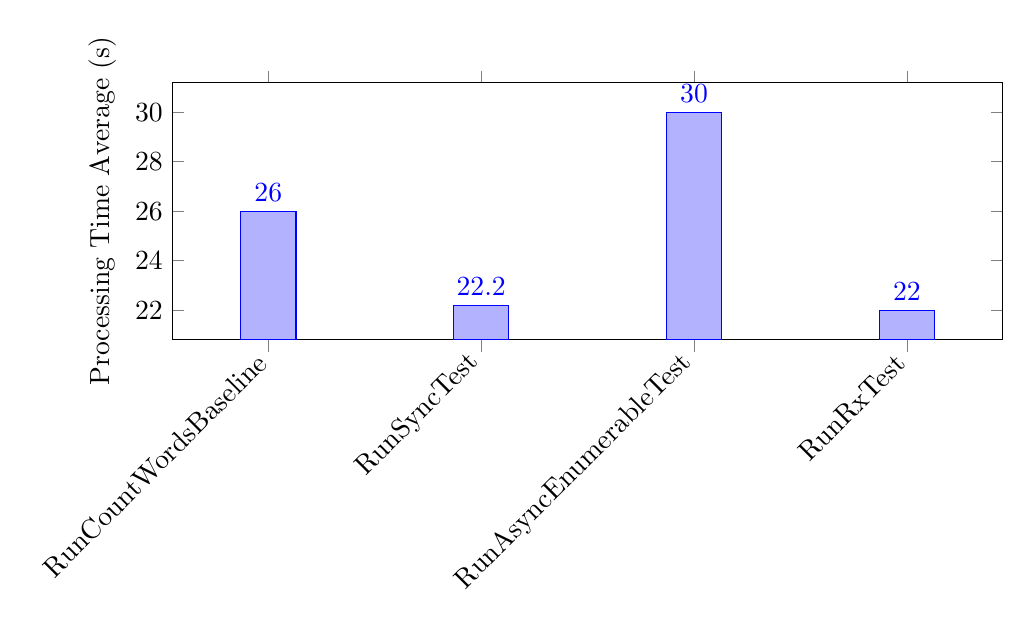
\begin{tikzpicture}
    \begin{axis}[
        ybar=2*\pgflinewidth,
        width=1.0\textwidth,
        height=0.4\textwidth,
        bar width=20pt,
        enlargelimits=0.15,
        legend style={at={(0.5,-0.2)}, anchor=north, legend columns=-1},
        ylabel={Processing Time Average (s)},
        symbolic x coords={RunCountWordsBaseline, RunSyncTest, RunAsyncEnumerableTest, RunRxTest},
        xtick=data,
        xticklabel style={rotate=45,anchor=east},
        nodes near coords,
        nodes near coords align={vertical},
        ]
    \addplot coordinates {(RunCountWordsBaseline, 26.0) (RunSyncTest, 22.2) (RunAsyncEnumerableTest, 30) (RunRxTest, 22.0)};
    \end{axis}
    \end{tikzpicture}
    \caption{Processing times for different strategies for "Count Words".}
    \label{fig:group_word_processing_times_cs}
\end{figure}



\section{Java/Kotlin Implementation}
\label{sec:java_implementation}

In this section, we will present the different strategies utilized in Java and Kotlin implementations for file processing and compare their performances. In the case of Java, asynchronous file reading isn't directly supported by the standard libraries. To overcome this limitation and maintain parity with the other implementations, we made use of a library named \texttt{AsyncFiles}. This library was developed by Professor Jorge Martins of the Lisbon Engineering Superior Institute. It provides an efficient and straightforward way to perform asynchronous file reading operations in Java.


\subsection{Results}
\label{subsubsec:results}

\subsubsection{Biggest Word Results}
\label{subsubsec:biggest_word_results}

\begin{table}[H]
    \centering
    \resizebox{\textwidth}{!}{%
    \begin{tabular}{|l|c|}
    \hline
    \textbf{Strategy} & \textbf{Processing Time Average (s)} \\ \hline
    NIO Reactor Flux & 1.1\\ \hline
    NIO Reactor Flux with Concurrency (use of \texttt{parallel()}) & 1.0 \\ \hline
    NIO Observable RXJava & 0.9 \\ \hline
    NIO Observable with Concurrency (use of \texttt{parallel()})& 0.8 \\ \hline
    Blocking Reader in Streams & 3.9 \\ \hline
    Blocking Reader MultiThread  & 0.7 \\ \hline
    Blocking Reader Streams with Concurrency & 3.0 \\ \hline
    NIO Baseline & 0.9 \\ \hline
    Concurrent Processing with Kotlin Flow & 2.4 \\ \hline
    Sequential Processing with Kotlin Flow & 5.1 \\ \hline
    Kotlin Flow IO Blocking Operations & 5.2 \\ \hline
    \end{tabular}%
    }
    \caption{Processing times for different Java/Kotlin strategies for "Biggest Word".}
    \label{tab:strategies_times_biggest_word}
    \end{table}
    
   
    \begin{figure}[H]
        \raggedright
        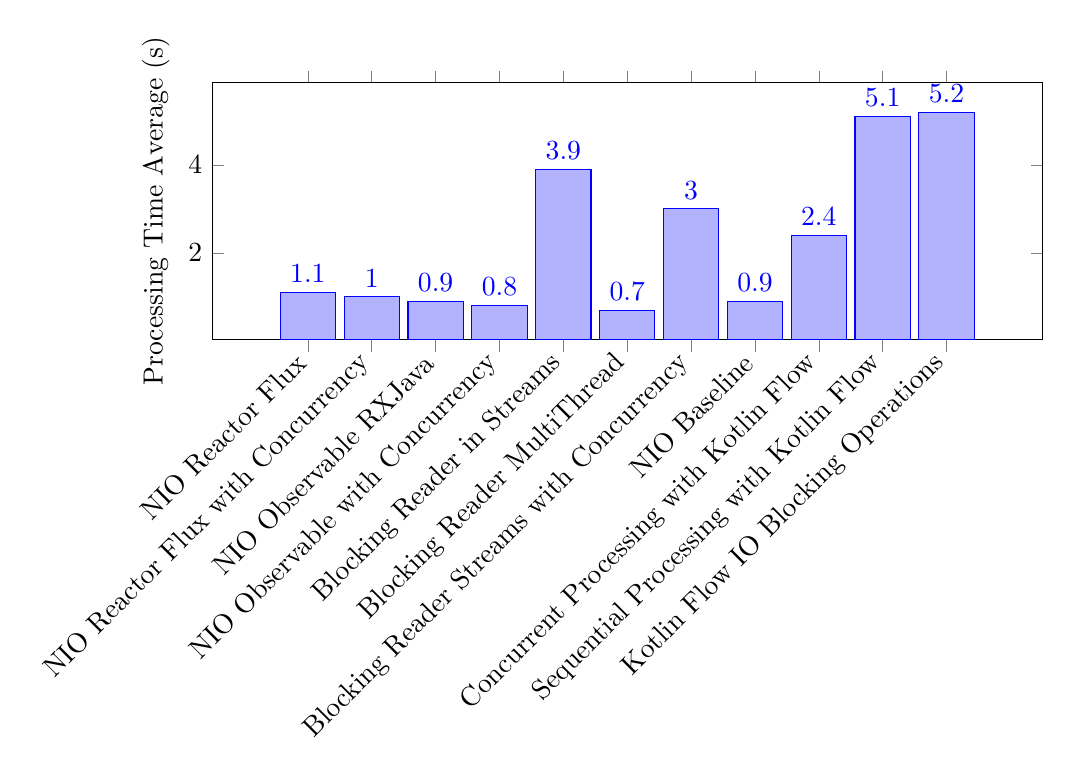
\begin{tikzpicture}
        \begin{axis}[
            ybar=2*\pgflinewidth,
            width=1.0\textwidth,
            height=0.4\textwidth,
            bar width=20pt,
            enlargelimits=0.15,
            legend style={at={(0.5,-0.2)}, anchor=north, legend columns=-1},
            ylabel={Processing Time Average (s)},
            symbolic x coords={NIO Reactor Flux, NIO Reactor Flux with Concurrency, NIO Observable RXJava, NIO Observable with Concurrency, Blocking Reader in Streams, Blocking Reader MultiThread, Blocking Reader Streams with Concurrency, NIO Baseline, Concurrent Processing with Kotlin Flow, Sequential Processing with Kotlin Flow, Kotlin Flow IO Blocking Operations},
            xtick=data,
            xticklabel style={rotate=45,anchor=east},
            nodes near coords,
            nodes near coords align={vertical},
            ]
        \addplot coordinates {(NIO Reactor Flux, 1.1) (NIO Reactor Flux with Concurrency, 1.0) (NIO Observable RXJava, 0.9) (NIO Observable with Concurrency, 0.8) (Blocking Reader in Streams, 3.9) (Blocking Reader MultiThread, 0.7) (Blocking Reader Streams with Concurrency, 3.0) (NIO Baseline, 0.9) (Concurrent Processing with Kotlin Flow, 2.4) (Sequential Processing with Kotlin Flow, 5.1) (Kotlin Flow IO Blocking Operations, 5.2)};
        \end{axis}
        \end{tikzpicture}
        \caption{Processing times for different Java/Kotlin strategies for "Biggest Word".}
        \label{fig:biggest_word_processing_times}
    \end{figure}
    

    
    \subsubsection{Group Word Results}
    \label{subsubsec:group_word_results}
    
    \begin{table}[H]
        \centering
        \resizebox{\textwidth}{!}{%
        \begin{tabular}{|l|c|}
        \hline
        \textbf{Strategy} & \textbf{Processing Time Average (s)} \\ \hline
        GroupWordsBaseline & 1.3 \\ \hline
        GroupWordsRXJava & 5.8 \\ \hline
        GroupWordsInRectorCoreFlux & 12.0 \\ \hline
        GroupWordsBlockingReaderInMultiThread & 1.2 \\ \hline
        GroupWordsBlockingReaderInStreams & 1.8 \\ \hline
        GroupWordsWithFlow (Kotlin) & 15.0\\ \hline
        \end{tabular}%
        }
        \caption{Processing times for different Java/Kotlin strategies for "Group Words".}
        \label{tab:strategies_times_group_words}
    \end{table}
        
    \begin{figure}[H]
        \centering
        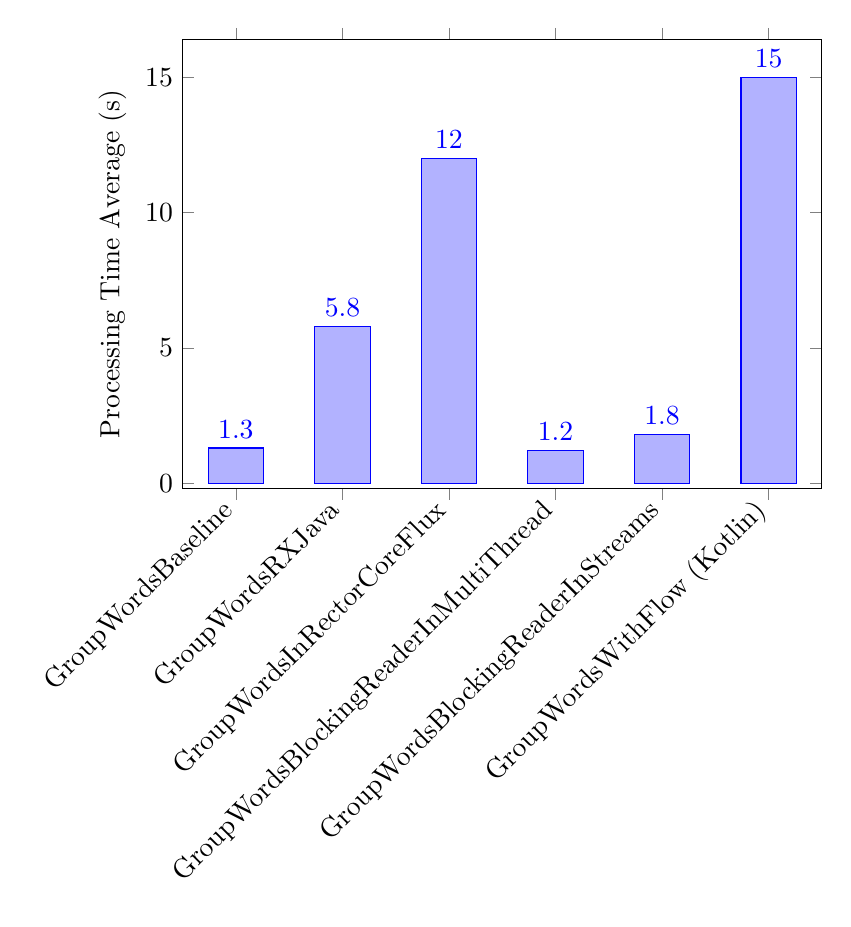
\begin{tikzpicture}
        \begin{axis}[
            ybar=2*\pgflinewidth,
            width=0.8\textwidth,
            height=0.6\textwidth,
            bar width=20pt,
            enlargelimits=0.10,
            legend style={at={(0.5,-0.2)}, anchor=north, legend columns=-1},
            ylabel={Processing Time Average (s)},
            symbolic x coords={GroupWordsBaseline, GroupWordsRXJava, GroupWordsInRectorCoreFlux, GroupWordsBlockingReaderInMultiThread, GroupWordsBlockingReaderInStreams, GroupWordsWithFlow (Kotlin)},
            xtick=data,
            xticklabel style={rotate=45,anchor=east},
            nodes near coords,
            nodes near coords align={vertical},
            ]
            \addplot coordinates { (GroupWordsBaseline, 1.3)  (GroupWordsRXJava, 5.8) (GroupWordsInRectorCoreFlux, 12.0) (GroupWordsBlockingReaderInMultiThread, 1.2)  (GroupWordsBlockingReaderInStreams, 1.8) (GroupWordsWithFlow (Kotlin), 15.0)};
        \end{axis}
        \end{tikzpicture}
        \caption{Processing times for different Java/Kotlin strategies for "Group Words".}
        \label{fig:processing_times}
    \end{figure}

... 
% Here you conclude the entire chapter by summarizing your findings and interpretations.


\section{JavaScript Implementation}
\label{sec:js_implementation}
\begin{table}[H]
    \centering
    \resizebox{\textwidth}{!}{%
    \begin{tabular}{|l|c|}
    \hline
    \textbf{Strategy} & \textbf{Processing Time Average (s)} \\ \hline
    Baseline JS & 8.2 \\ \hline
    Baseline Stream JS & 23.2 \\ \hline
    RxStrategy JS & 13.9 \\ \hline
    \end{tabular}%
    }
    \caption{Processing times for different JavaScript strategies for "Biggest Word".}
    \label{tab:strategies_times_biggest_word_js}
\end{table}

\begin{figure}[H]
    \raggedright
    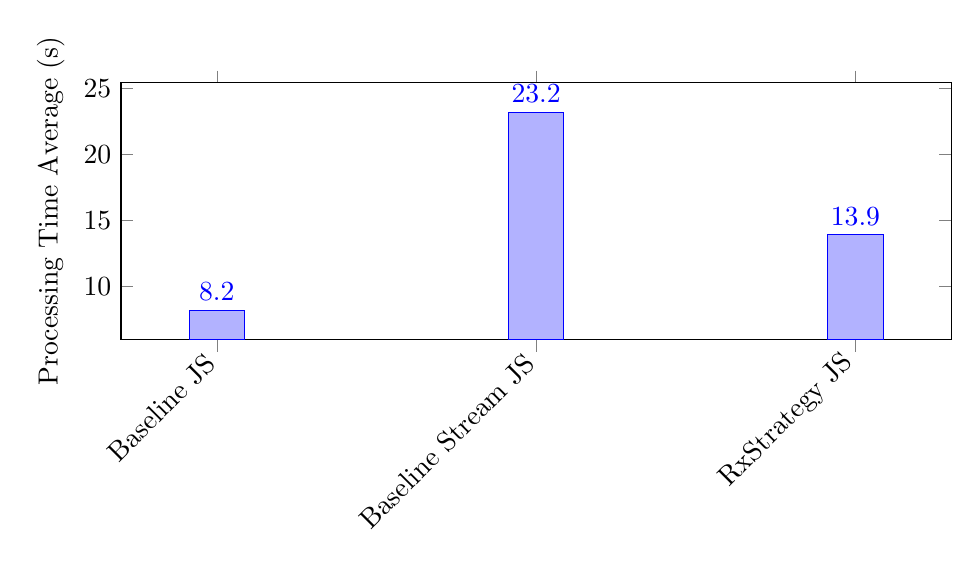
\begin{tikzpicture}
    \begin{axis}[
        ybar=2*\pgflinewidth,
        width=1.0\textwidth,
        height=0.4\textwidth,
        bar width=20pt,
        enlargelimits=0.15,
        legend style={at={(0.5,-0.2)}, anchor=north, legend columns=-1},
        ylabel={Processing Time Average (s)},
        symbolic x coords={Baseline JS, Baseline Stream JS, RxStrategy JS},
        xtick=data,
        xticklabel style={rotate=45,anchor=east},
        nodes near coords,
        nodes near coords align={vertical},
        ]
    \addplot coordinates {(Baseline JS, 8.2) (Baseline Stream JS, 23.2) (RxStrategy JS, 13.9)};
    \end{axis}
    \end{tikzpicture}
    \caption{Processing times for different JavaScript strategies for "Biggest Word" Graphic}
    \label{fig:biggest_word_processing_times_js}
\end{figure}



\subsection{Discussion}
\label{subsec:discussion}

% Here you discuss the results, as you did in the provided document.



\section{Conclusion}
\label{sec:conclusion}

\end{document}